\section{\textbf{Comparison with Other Approaches}}

To assess how the AMEN approach compares with alternatives in the literature we utilize the same network dataset used by \citet{cranmer:etal:2016}. Their application utilizes a cross-sectional network measuring whether an actor indicated that they collaborated with another during the policy design of the Swiss CO$_{2}$ act \citep{ingold:2008}.\footnote{This is a directed relational matrix as an actor $i$ can indicate that they collaborated with $j$ but $j$ may not have stated that they collaborated with $i$.} The Swiss government proposed this act in 1995 with the goal of undertaking a 10\% reduction in CO$_{2}$ emissions by 2012. The act was accepted in the Swiss Parliament in 2000 and implemented in 2008. \citet{ingold:2008}, and subsequent work by \citet{ingold:fischer:2014}, sought to determine what drives collaboration among actors trying to affect climate change policy. The set of actors included in this network are those that were identified by experts as holding an important position in Swiss climate policy.\footnote{For further details on the methodology utilized in choosing the set of actors see \citet{ingold:2008,ingold:fischer:2014}.} In total, \citet{ingold:2008} identifies 34 relevant actors: five state actors, eleven industry and business representatives, seven environmental NGOs and civil society organizations, five political parties, and six scientific institutions and consultants. 

\begin{figure}[ht]
	\centering
	\begin{tabular}{cc}
	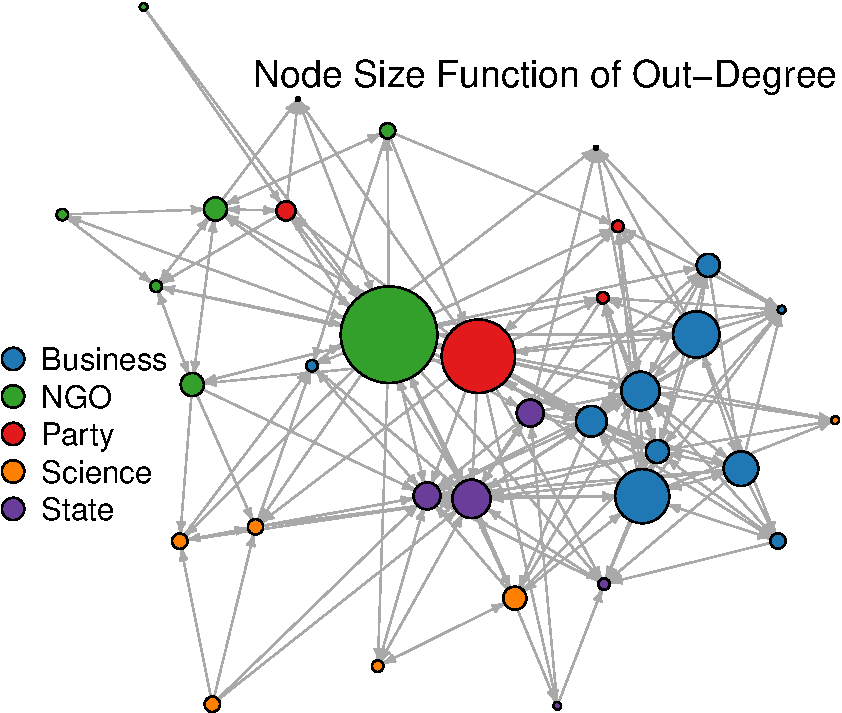
\includegraphics[width=.47\textwidth]{dvNet_outDegree} & 
	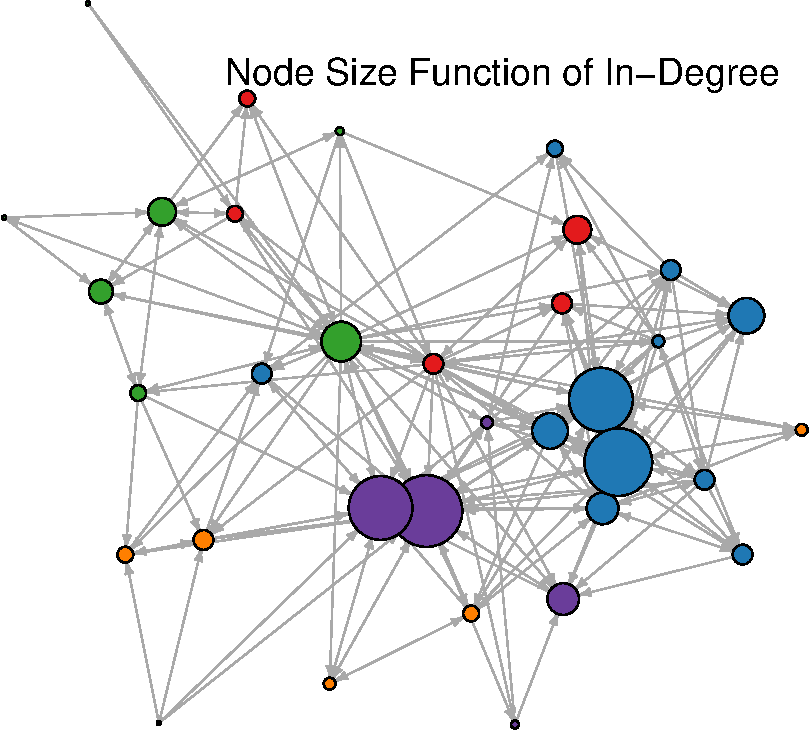
\includegraphics[width=.44\textwidth]{dvNet_inDegree}
	\end{tabular}
	\caption{Network visualizations of the Swiss climate change mitigation network. Nodes are colored by type of actor, and directed edges indicate relationships between actors. The network on the left weights node size by the number of out-going ties, and on the right the number of incoming-ties.}
	\label{fig:dvNet}
\end{figure}
\FloatBarrier

Figure~\ref{fig:dvNet} provides a pair of visualizations for this directed collaboration network. Nodes are colored by the type of actor and a directed edge indicates an actor stated that they collaborated with another, and determining which actor indicated the collaboration can be ascertained by the direction of the arrow. The positions of actors in these networks is estimated using a force-directed layout algorithm.\footnote{To determine the positions of nodes in this network we use the Fruchterman-Reingold algorithm \citep{fruchterman:reingold:1991}.} These types of algorithms use information contained within the structure of the network itself to provide informative depictions of graphs. A straightforward way to understand how they work is to think of nodes connected by edges as particles that are attracted to each other, and nodes that are unconnected as particles that repulse each other. These types of algorithms simulate a system in which nodes pull and push upon each other until they reach an equilibrium position. In this case, the algorithm provides us with some useful information about relationships between nodes. Specifically, we see that the majority of the industry and business actors are clustering together, meaning that these types of actors tend to indicate they collaborated with one another during the policy design process. We can also see that three of the state actors are pushed towards the center of the graph by the algorithm, which occurs because they share relationships with a variety of types of actors. Most of the actors classified as scientific institutions are pushed towards the far left border of the graphs as it seems they tend to interact amongst themselves and just a few of the other types of actors. 

An important part of our discussion from the previous section revolved around the idea that within network structures we find variation in how active nodes are in engaging with others in the network. To illustrate nodal heterogeneity in the case of the Swiss climate change mitigation networks we weight the size of nodes, in the network on the left, by the number of their outgoing ties, and on the right by their incoming ties. From the network on the left, it is clear that some nodes are much more likely to indicate that they formed collaborations with others. For example, each of the scientific institutions and consultants shown in Figure~\ref{fig:dvNet} indicate that they collaborate with relatively few organizations, especially, as compared to actors from industry and business. Additionally, there is even variation within actor types as evidenced by differences amongst NGO or political party actors. Similar findings of nodal heterogeneity emerge if we turn our attention to examining nodes by their incoming ties. 

% The cursory discussion above regarding nodal heterogeneity should already point to the importance of taking into account lower order interdependencies between observations, and given the higher order structure  
Obvious from an examination of Figure~\ref{fig:dvNet} is that collaboration among these 34 actors is not simply a function of actor type. To understand what factors may play a role in shaping collaboration in this relational data structure a modeling approach is necessary, and based on our discussion from the previous section we would argue that, specifically, a network analytic procedure is required. \citet{cranmer:etal:2016} follow \citet{ingold:fischer:2014} in developing a model specification. We do not review the specification in detail here, instead we just provide a summary of the variables to be included and the theoretical expectations of their effects in Table~\ref{tab:theorySpec}. 

\newcolumntype{L}{>{\arraybackslash}m{9cm}}
\begin{table}[ht]
\centering
\begingroup\scriptsize
\begin{tabular}{lLc}
\footnotesize{\textbf{Variable}} & \footnotesize{\textbf{Description}} & \footnotesize{\textbf{Expected Effect}} \\ \hline\hline
	\multicolumn{3}{l}{\textbf{Conflicting policy preferences}} \\ 
	\quad Business v. NGO & Binary, dyadic covariate that equals one when one actor is from the business sector and the other an NGO & $-$ \\
	\quad Opposition/alliance & Binary, dyadic covariate that equals one when $i$, sender, perceives $j$, receiver, as having similar policy objectives regarding climate change  & $+$ \\
	\quad Preference dissimilarity & Transformation of four core beliefs into a Manhattan distance matrix, smaller the distance the closer the beliefs of $i$ and $j$ & $-$ \\ 
	\multicolumn{3}{l}{\textbf{Transaction costs}} \\ 
	\quad Joint forum participation & Binary, dyadic covariate that equals one when $i$ and $j$ belong to the same policy forum & $+$ \\ 
	\multicolumn{3}{l}{\textbf{Influence}} \\ 
	\quad Influence attribution & Binary, dyadic covariate that equals one when $i$ considers $j$ to be influential & $+$ \\
	\quad Alter's influence in-degree & Number of actors that mention $i$ as being influential, this is a measure of reputational power & $+$ \\
	\quad Influence absolute diff. & Absolute difference in reputational power between $i$ and $j$ & $-$ \\
	\quad Alter = Government Actor & Binary, nodal covariate that equals one when $j$ is a state actor & $+$ \\ 
	\multicolumn{3}{l}{\textbf{Functional requirements}} \\ 
	\quad Ego = Environment NGO & Binary, nodal covariate that equals one when $i$ is an NGO & $+$ \\
	\quad Same actor type & Binary, dyadic covariate that equals when $i$ and $j$ are the same actor type & $+$ \\ 
	\multicolumn{3}{l}{\textbf{Endogenous dependencies: ERGM Specific Parameters}} \\ 
	\quad Mutuality & Captures concept of reciprocity, if $i$ indicates they collaborated with $j$ then $j$ likely collaborates with $i$ & $+$\\
	\quad Outdegree popularity & Captures idea that actors sending more ties will be more popular targets themselves for collaboration  & $+$ \\
	\quad Twopaths & Counts the number of two-paths in the network, two-path is an instance where $i$ is connected to $j$, $j$ to $k$, but $i$ is not connected to $k$ & $-$ \\
	\quad GWIdegree (2.0) & Captures how many ties a node sends in the network, used to capture networks with some nodes that are highly active  & $+$ \\
	\quad GWESP (1.0) & Counts the number of shared partners for each pair and sums across  & $+$ \\
	\quad GWOdegree (0.5) & Captures how many ties a node receives in the network, used to capture networks with some nodes that are highly popular  & $+$ \\
\hline\hline
\end{tabular}
\endgroup
\caption{Summary of variables to be included in model specification. With the exception of mutuality, each of the parameters falling in the Endogenous dependencies grouping are only explicitly testable through ERGM. }
\label{tab:theorySpec}
\end{table}
\FloatBarrier

\subsection{Parameter Estimates}

Using the specification described in Table~\ref{tab:theorySpec} we compare five different modeling approaches. The first two approaches are a simple logistic model and the MRQAP.  

% latex table generated in R 3.3.1 by xtable 1.8-2 package
% Sun Aug 21 03:32:43 2016
\begin{table}[ht]
\centering
\begingroup\normalsize
\begin{tabular}{lccccc}
   & Logit & MRQAP & LSM & ERGM & AME \\ 
  \hline
\hline
Intercept/Edges & -4.44$^{\ast}$ & -4.24$^{\ast}$ & 0.94$^{\ast}$ & -12.17$^{\ast}$ & -3.39$^{\ast}$ \\ 
   & (0.34) &  & [0.09; 1.82] & (1.40) & [-4.38; -2.50] \\ 
  \textbf{Conflicting policy preferences} &  &  &  &  &  \\ 
  $\;\;\;\;$ Business vs. NGO & -0.86 & -0.87$^{\ast}$ & -1.37$^{\ast}$ & -1.11$^{\ast}$ & -1.37$^{\ast}$ \\ 
   & (0.46) &  & [-2.42; -0.41] & (0.51) & [-2.44; -0.47] \\ 
  $\;\;\;\;$ Opposition/alliance & 1.21$^{\ast}$ & 1.14$^{\ast}$ & 0.00 & 1.22$^{\ast}$ & 1.08$^{\ast}$ \\ 
   & (0.20) &  & [-0.40; 0.39] & (0.20) & [0.72; 1.47] \\ 
  $\;\;\;\;$ Preference dissimilarity & -0.07 & -0.60 & -1.76$^{\ast}$ & -0.44 & -0.79$^{\ast}$ \\ 
   & (0.37) &  & [-2.62; -0.90] & (0.39) & [-1.55; -0.08] \\ 
  \textbf{Transaction costs} &  &  &  &  &  \\ 
  $\;\;\;\;$ Joint forum participation & 0.88$^{\ast}$ & 0.75$^{\ast}$ & 1.51$^{\ast}$ & 0.90$^{\ast}$ & 0.92$^{\ast}$ \\ 
   & (0.27) &  & [0.86; 2.17] & (0.28) & [0.40; 1.47] \\ 
  \textbf{Influence} &  &  &  &  &  \\ 
  $\;\;\;\;$ Influence attribution & 1.20$^{\ast}$ & 1.29$^{\ast}$ & 0.08 & 1.00$^{\ast}$ & 1.09$^{\ast}$ \\ 
   & (0.22) &  & [-0.40; 0.55] & (0.21) & [0.69; 1.53] \\ 
  $\;\;\;\;$ Alter's influence indegree & 0.10$^{\ast}$ & 0.11$^{\ast}$ & 0.01 & 0.21$^{\ast}$ & 0.11$^{\ast}$ \\ 
   & (0.02) &  & [-0.03; 0.04] & (0.04) & [0.07; 0.15] \\ 
  $\;\;\;\;$ Influence absolute diff. & -0.03$^{\ast}$ & -0.06$^{\ast}$ & 0.04 & -0.05$^{\ast}$ & -0.07$^{\ast}$ \\ 
   & (0.02) &  & [-0.01; 0.09] & (0.01) & [-0.11; -0.03] \\ 
  $\;\;\;\;$ Alter = Government actor & 0.63$^{\ast}$ & 0.68 & -0.46 & 1.04$^{\ast}$ & 0.55 \\ 
   & (0.25) &  & [-1.08; 0.14] & (0.34) & [-0.07; 1.15] \\ 
  \textbf{Functional requirements} &  &  &  &  &  \\ 
  $\;\;\;\;$ Ego = Environmental NGO & 0.88$^{\ast}$ & 0.99 & -0.60 & 0.79$^{\ast}$ & 0.67 \\ 
   & (0.26) &  & [-1.32; 0.09] & (0.17) & [-0.38; 1.71] \\ 
  $\;\;\;\;$ Same actor type & 0.74$^{\ast}$ & 1.12$^{\ast}$ & 1.17$^{\ast}$ & 0.99$^{\ast}$ & 1.04$^{\ast}$ \\ 
   & (0.22) &  & [0.63; 1.71] & (0.23) & [0.63; 1.50] \\ 
  \textbf{Endogenous dependencies} &  &  &  &  &  \\ 
  $\;\;\;\;$ Mutuality & 1.22$^{\ast}$ & 1.00$^{\ast}$ &  & 0.81$^{\ast}$ & 0.39 \\ 
   & (0.21) &  &  & (0.25) & [-0.12; 0.96] \\ 
  $\;\;\;\;$ Outdegree popularity &  &  &  & 0.95$^{\ast}$ &  \\ 
   &  &  &  & (0.09) &  \\ 
  $\;\;\;\;$ Twopaths &  &  &  & -0.04$^{\ast}$ &  \\ 
   &  &  &  & (0.02) &  \\ 
  $\;\;\;\;$ GWIdegree (2.0) &  &  &  & 3.42$^{\ast}$ &  \\ 
   &  &  &  & (1.47) &  \\ 
  $\;\;\;\;$ GWESP (1.0) &  &  &  & 0.58$^{\ast}$ &  \\ 
   &  &  &  & (0.16) &  \\ 
  $\;\;\;\;$ GWOdegree (0.5) &  &  &  & 8.42$^{\ast}$ &  \\ 
   &  &  &  & (2.11) &  \\ 
   \hline
\hline
\end{tabular}
\endgroup
\caption{* p $<$ 0.05. Logistic regression and ERGM results are shown with standard errors in parentheses. MRQAP provides no standard errors. LSM and AME are shown with 95\% posterior credible intervals provided in brackets.} 
\label{tab:regTable}
\end{table}

\FloatBarrier

\subsection{Tie Formation Prediction}

The results are displayed in Figure \ref{fig:roc} using separation plots and Receiver Operating Characteristic (ROC) curves.

We compare the sensitivity and specificity trade-off for each model using ROC curves. Models that have a better fit according to this test should have curves that follow the left-hand border and then the top border of the ROC space. Here again it is apparent that accounting for the interstate relations and the endogenous network effects leads to noticeable improvements in performance. Last, by calculating the area under the ROC curve (AUC) we can assess the accuracy of each model.

Separation plots provide a visual interpretation of model fit by plotting all observations, in this case country pairs, in the data set according to their predicted value from left (low values) to right (high values). Models with a good fit should should have all actual (dark blue) observations towards the right of the separation plot \citep{greenhill:etal:2011}.

In addition, we also highlight the difference in performance through the utilization of a precision-recall curve. Precision is a measure of result relevancy, while recall is a measure of how many truly relevant results are returned. A high area under the curve represents both high recall and high precision, where high precision relates to a low false positive rate, and high recall relates to a low false negative rate. High scores for both show that the classifier is returning accurate results (high precision), as well as returning a majority of all positive results (high recall). 

Precision is defined as the number of true positives over the number of true positives plus the number of false positives. 

Recall is defined as the number of true positives over the number of true positives plus the number of false negatives. 

\begin{figure}[ht]
	\centering
	\begin{tabular}{cc}
	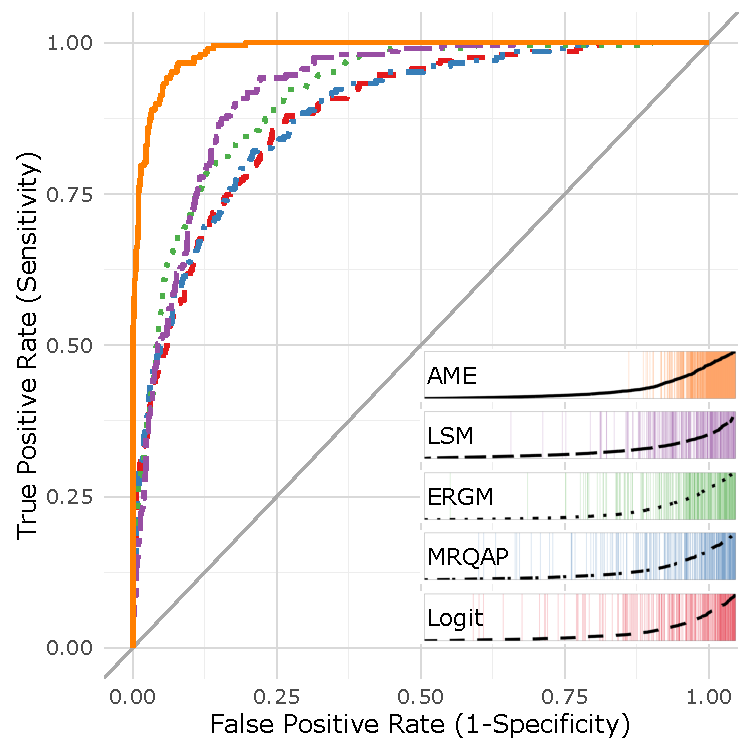
\includegraphics[width=.5\textwidth]{roc} & 
	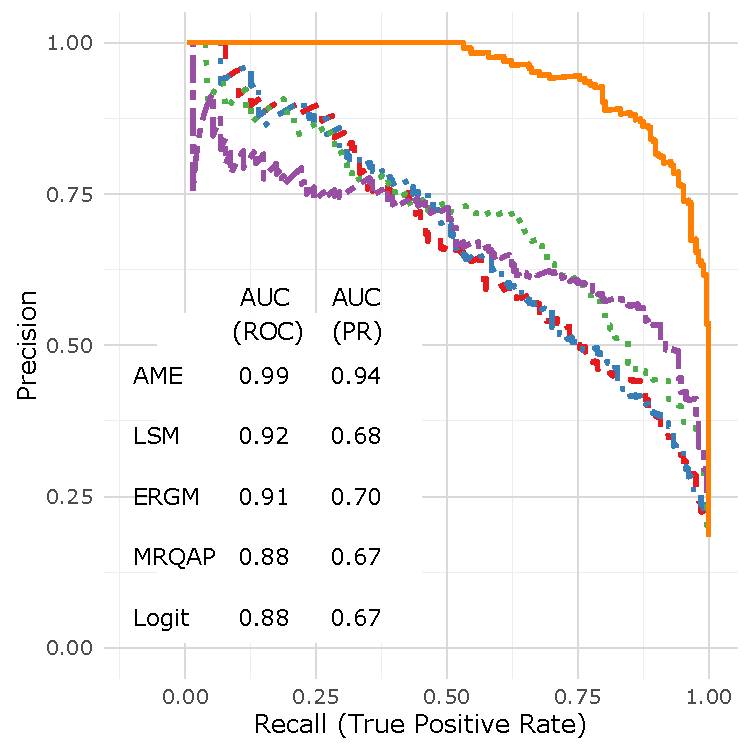
\includegraphics[width=.5\textwidth]{rocPr}	
	\end{tabular}
	\caption{ROC and separation plots}
	\label{fig:roc}
\end{figure}
\FloatBarrier

\subsection{Capturing Network Attributes}

To assess whether the model adequately captures the network parameters of the DV. Here we compare the observed with a set of simulated networks based on certain network statistics \citep{hunter:etal:2008}. 

See \citet{morris:etal:2008} for details on each of these parameters. 

\begin{itemize}
\item Dyad-wise shared partners - Number of dyads in the network with exactly $i$ shared partners
\item Edge-wise shared partners - Similar to above except this counts the number of dyads with the same number of edges
\item Geodesic distances - The proportion of pairs of nodes whose shortest connecting path is of length $k$, for $k=1,2,\ldots$ Also, pairs of nodes that are not connected are classified as $k=\infty$.
\item Incoming k-star - Propensities for individuals to have connections with multiple network partners
\item Indegree - degree count is the number of nodes with the same value of the attribute as the ego node
\item Outdegree - degree count is the number of nodes with the same value of the attribute as the ego node
\end{itemize}

\begin{figure}[ht]
	\centering
	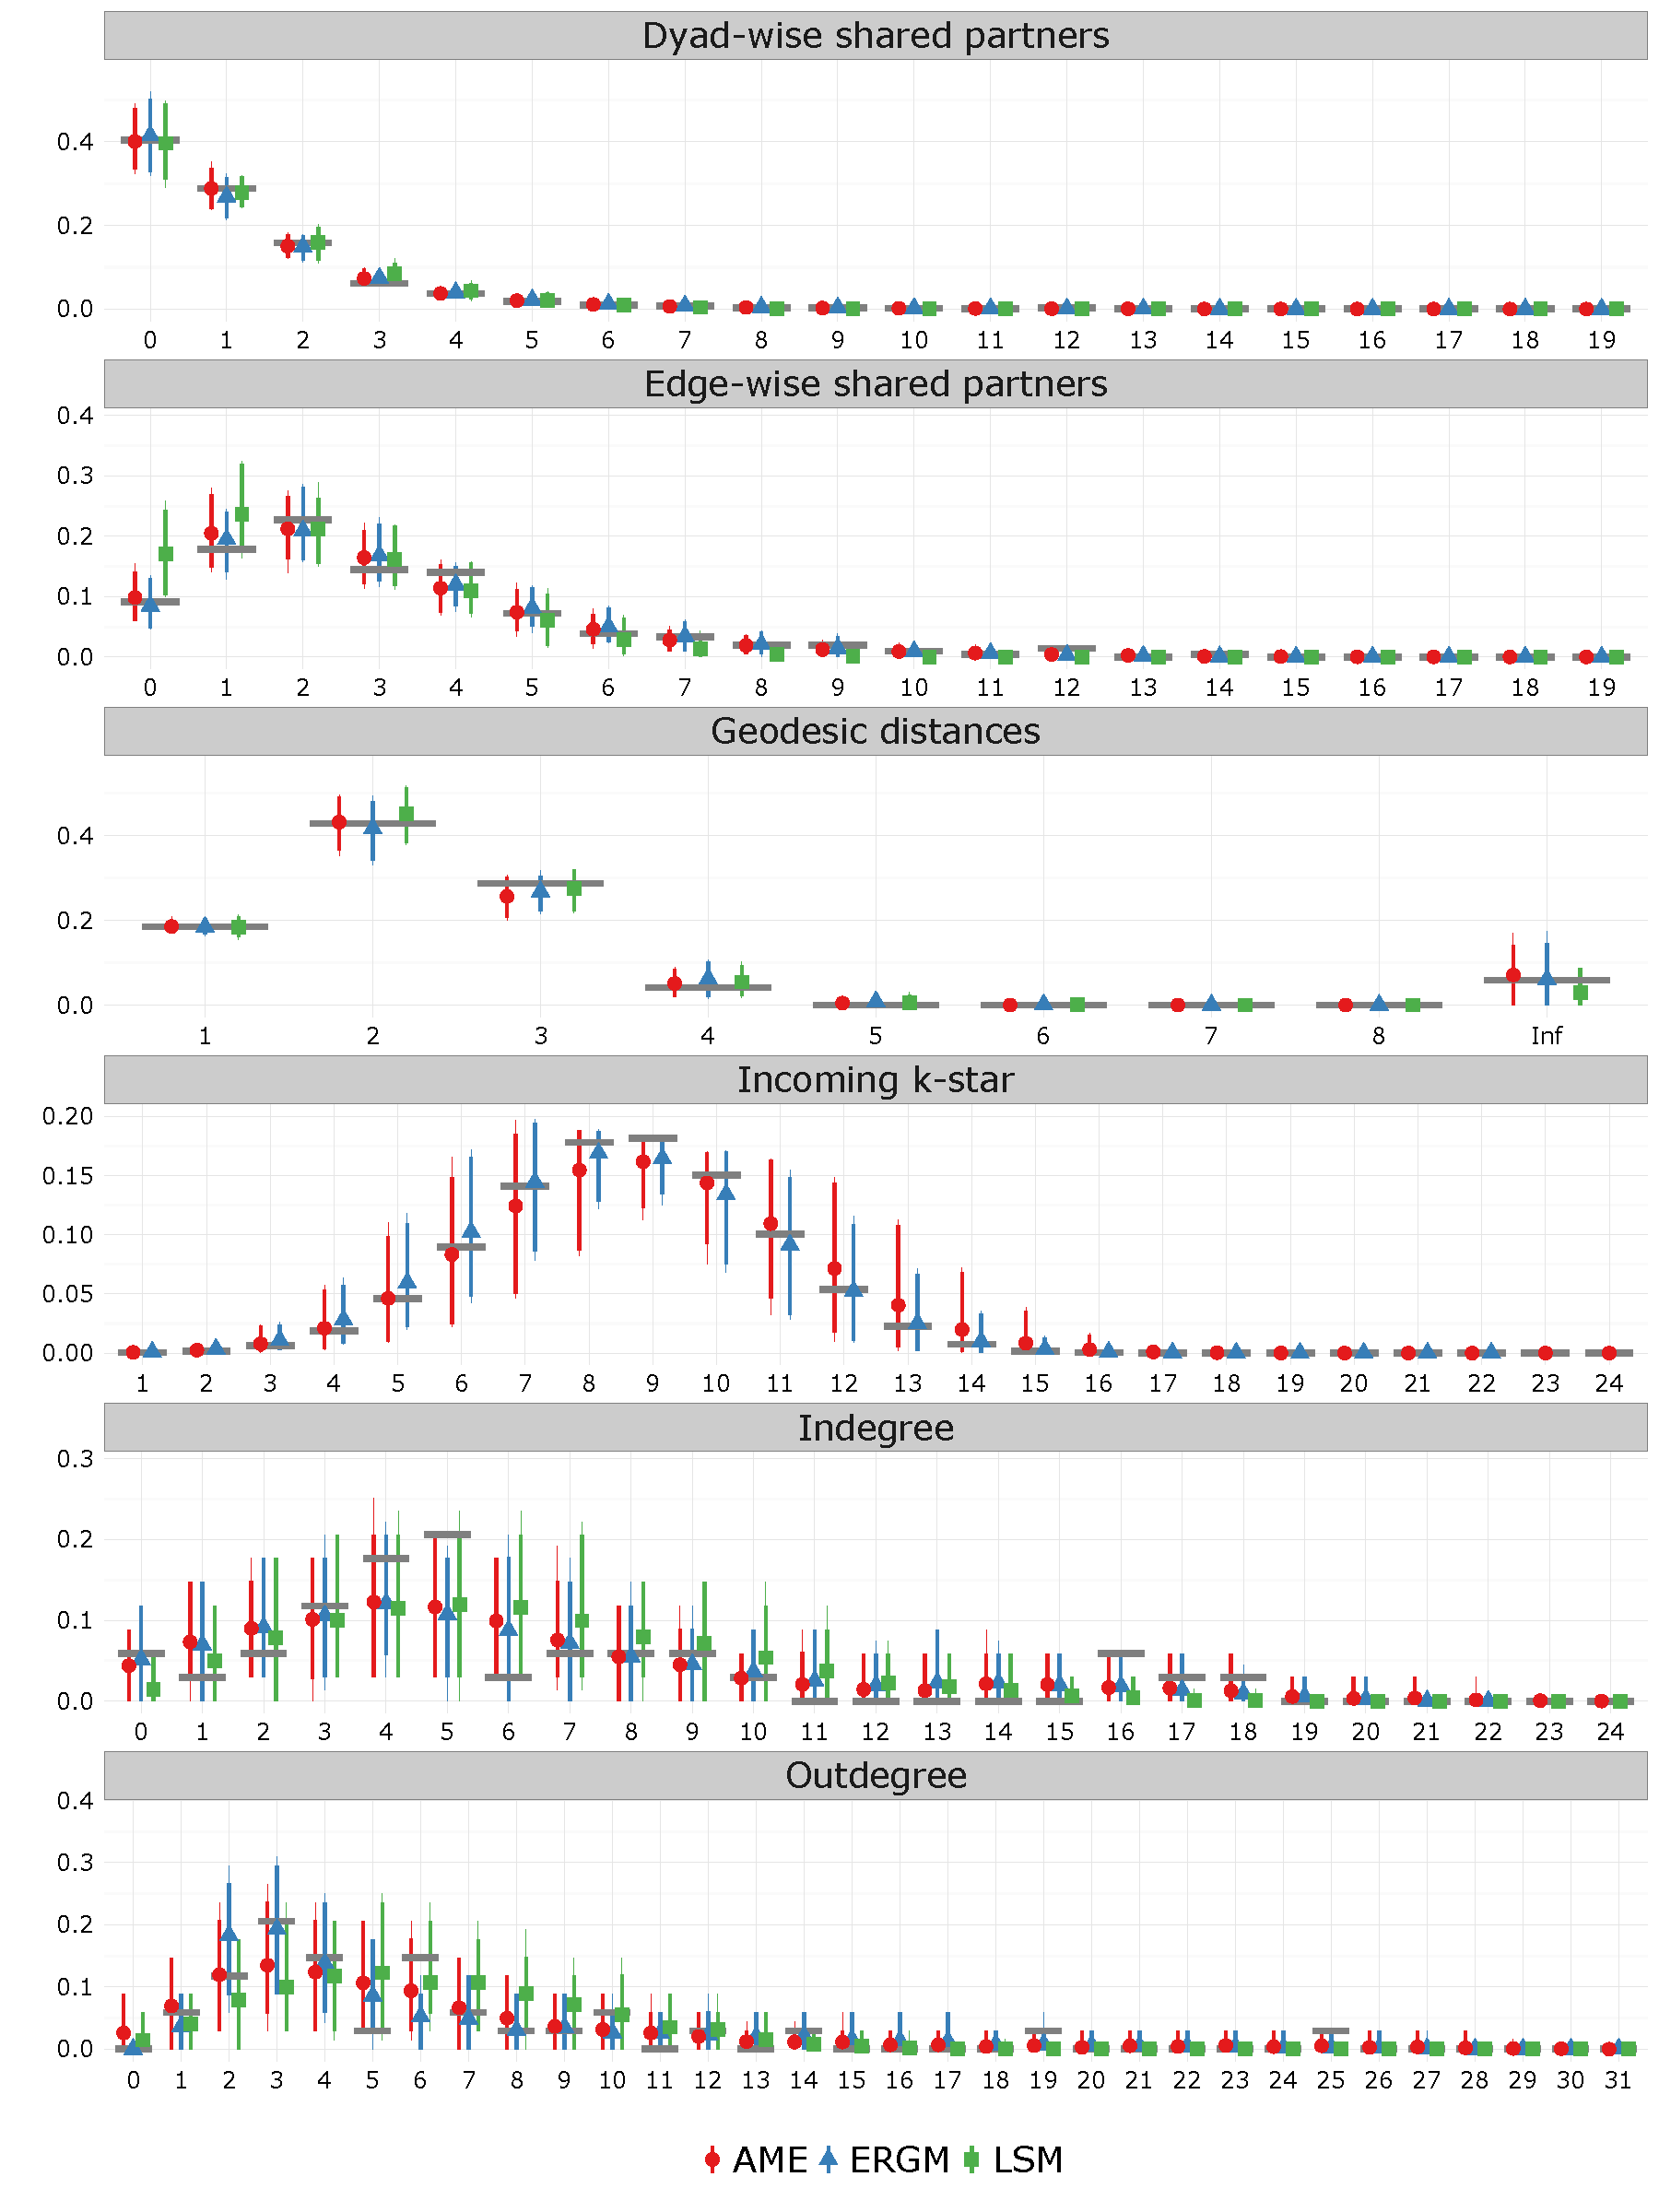
\includegraphics[width=1\textwidth]{ggGofAll}
	\caption{network stats }
	\label{fig:gofAll}
\end{figure}

Figure~\ref{fig:ergmAmePerf} give posterior predictive goodness of fit summaries for four network statistics: (1) the empirical standard deviation of the row means; (2) the empirical standard deviation of the column means (heterogeneity of nodes with incoming activity); (3) the empirical within-dyad correlation; (4) a normalized measure of triadic dependence \citep{hoff:etal:2015}. 

For a given summary statistic g() we first simulate $\mathbf{Y}_{sim} \approx p(\mathbf{Y}_{sim} | \mathbf{Y}_{obs}) = \int p(\mathbf{Y}_{sim} | \theta) p(d \theta | \mathbf{Y}_{obs})$ and then we compare $g(\mathbf{Y}_{sim})$ to $g(\mathbf{Y}_{obs})$. Histograms represent predicted value of statistics under the model and red dash line represents the observed value. 

Proportion of ties that are reciprocated. 

\begin{align}
\begin{aligned}
t(Y) &= \frac{ \sum_{i \neq j}y_{i,j} y_{j,i} }{ \sum_{i \neq j} y_{i,j} } \\
\end{aligned}
\end{align}

Number of transitive triplets, number of triangles in network, number of times ijk are all connected.

\begin{align}
\begin{aligned}
t(Y) &= \sum_{i \neq j \neq k} y_{i,j} y_{i,k} y_{j,k}
\end{aligned}
\end{align}

\begin{figure}[ht]
	\centering
	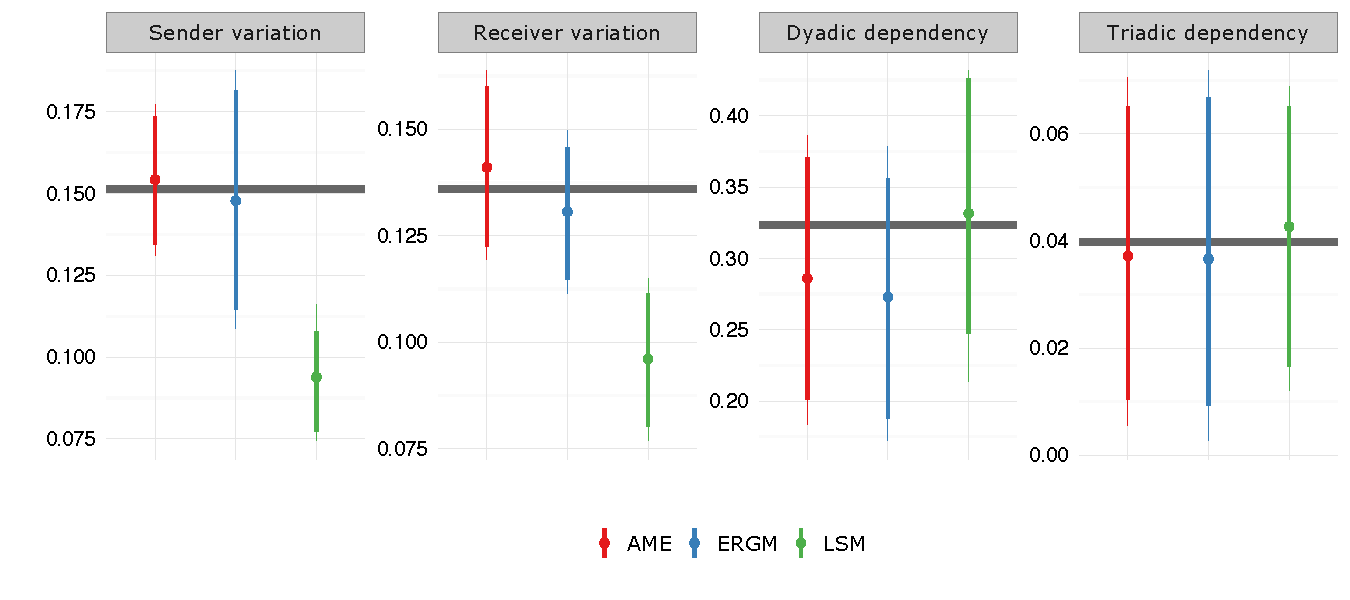
\includegraphics[width=1\textwidth]{netPerfCoef}
	\caption{Posterior predictive goodness of fit summary}
	\label{fig:ergmAmePerf}
\end{figure}
\FloatBarrier